\documentclass[11pt]{article}
\usepackage[utf8]{inputenc}
\usepackage[T1]{fontenc}
\usepackage{amsmath}
\usepackage{amssymb}
\usepackage{multicol}
\usepackage{geometry}
\usepackage{tikz}
\usetikzlibrary{shapes,patterns,angles,quotes,calc}
\usepackage{enumitem}
\usepackage{xcolor}
\usepackage{titlesec}

% Configurações de layout
\geometry{a4paper, left=1cm, right=1cm, top=0.5cm, bottom=1.2cm}
\setlength{\columnseprule}{0.4pt}

% Cores para títulos
\titleformat{\section}{\normalfont\Large\bfseries\color{blue}}{\thesection}{1em}{}
\titleformat{\subsection}{\normalfont\large\bfseries\color{red}}{\thesubsection}{1em}{}

\title{\textcolor{red}{Geometria: Cálculo de Áreas
    \\Fórmulas e Aplicações}}
\author{Professor: Jefferson}
\date{}

\begin{document}

\maketitle
\vspace{-1cm}

%\begin{center}
%\large{Nome: \underline{\hspace{8cm}} \quad Turma: \underline{\hspace{3cm}}}
%\end{center}

\begin{multicols}{2}

\section*{Conceito de Área}

\textbf{Área} é a medida da superfície de uma figura plana, expressa em unidades quadradas (m², cm², etc.).

\subsection*{Unidades de Medida}
\begin{itemize}
\item km² (quilômetro quadrado)
\item m² (metro quadrado)
\item cm² (centímetro quadrado)
\item mm² (milímetro quadrado)
\end{itemize}

\section*{Fórmulas Fundamentais}

\subsection*{Quadrado}

\begin{center}
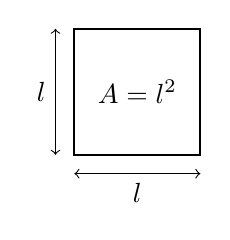
\begin{tikzpicture}[scale=0.8]
\draw[thick] (0,0) rectangle (2,2);
\draw[<->] (0,-0.3) -- (2,-0.3) node[midway,below] {$l$};
\draw[<->] (-0.3,0) -- (-0.3,2) node[midway,left] {$l$};
\node at (1,1) {$A = l^2$};
\end{tikzpicture}
\end{center}

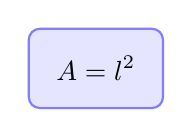
\begin{tikzpicture}
\node[rectangle, fill=blue!10, rounded corners, inner sep=10pt, draw=blue!50, thick] (box) {
$\displaystyle A = l^2$
};
\end{tikzpicture}

\textbf{Onde:}
\begin{itemize}
\item $l$ = medida do lado
\end{itemize}

\subsection*{Retângulo}

\begin{center}
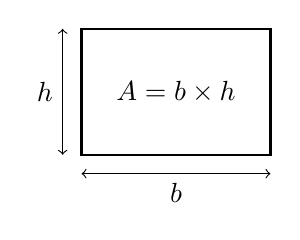
\begin{tikzpicture}[scale=0.8]
\draw[thick] (0,0) rectangle (3,2);
\draw[<->] (0,-0.3) -- (3,-0.3) node[midway,below] {$b$};
\draw[<->] (-0.3,0) -- (-0.3,2) node[midway,left] {$h$};
\node at (1.5,1) {$A = b \times h$};
\end{tikzpicture}
\end{center}

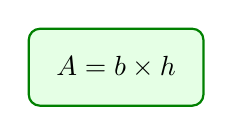
\begin{tikzpicture}
\node[rectangle, fill=green!10, rounded corners, inner sep=10pt, draw=green!50!black, thick] (box) {
$\displaystyle A = b \times h$
};
\end{tikzpicture}

\textbf{Onde:}
\begin{itemize}
\item $b$ = base
\item $h$ = altura
\end{itemize}

\subsection*{Triângulo}

\begin{center}
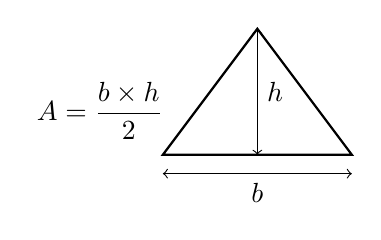
\begin{tikzpicture}[scale=0.8]
\draw[thick] (0,0) -- (3,0) -- (1.5,2) -- cycle;
\draw[dashed] (1.5,2) -- (1.5,0);
\draw[<->] (0,-0.3) -- (3,-0.3) node[midway,below] {$b$};
\draw[<->] (1.5,0) -- (1.5,2) node[midway,right] {$h$};
\node at (-1.0,0.7) {$A = \dfrac{b \times h}{2}$};
\end{tikzpicture}
\end{center}

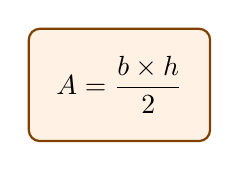
\begin{tikzpicture}
\node[rectangle, fill=orange!10, rounded corners, inner sep=10pt, draw=orange!50!black, thick] (box) {
$\displaystyle A = \frac{b \times h}{2}$
};
\end{tikzpicture}

\textbf{Outras fórmulas para triângulo:}
\begin{itemize}
\item Fórmula de Herão: $A = \sqrt{p(p-a)(p-b)(p-c)}$
  onde $p = \dfrac{a+b+c}{2}$ (semiperímetro)
\item Com dois lados e ângulo: $A = \dfrac{a \times b \times \sin\theta}{2}$
\end{itemize}

\subsection*{Paralelogramo}

\begin{center}
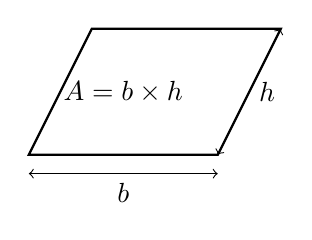
\begin{tikzpicture}[scale=0.8]
\draw[thick] (0,0) -- (3,0) -- (4,2) -- (1,2) -- cycle;
\draw[dashed] (0,0) -- (1,2);
\draw[<->] (0,-0.3) -- (3,-0.3) node[midway,below] {$b$};
\draw[<->] (3,0) -- (4,2) node[midway,right] {$h$};
\node at (1.5,1) {$A = b \times h$};
\end{tikzpicture}
\end{center}

\subsection*{Trapézio}

\begin{center}
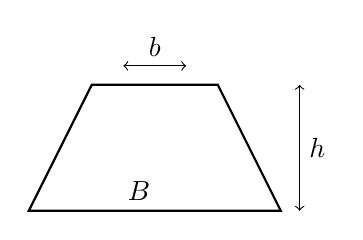
\begin{tikzpicture}[scale=0.8]
\draw[thick] (0,0) -- (4,0) -- (3,2) -- (1,2) -- cycle;
\draw[-] (1.5,0) -- (2,0) node[midway,above] {$B$};
\draw[<->] (1.5,2.3) -- (2.5,2.3) node[midway,above] {$b$};
\draw[<->] (4.3,0) -- (4.3,2) node[midway,right] {$h$};
\end{tikzpicture}
\end{center}

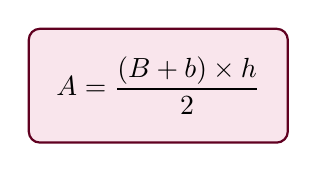
\begin{tikzpicture}
\node[rectangle, fill=purple!10, rounded corners, inner sep=10pt, draw=purple!50!black, thick] (box) {
$\displaystyle A = \frac{(B + b) \times h}{2}$
};
\end{tikzpicture}

\subsection*{Losango}

\begin{center}
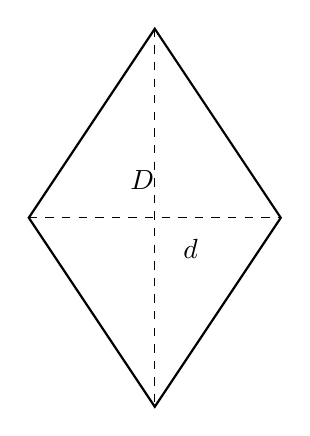
\begin{tikzpicture}[scale=0.8]
\draw[thick] (0,0) -- (2,3) -- (4,0) -- (2,-3) -- cycle;
\draw[dashed] (0,0) -- (4,0);
\draw[dashed] (2,3) -- (2,-3);
\draw (1.80,0.3) -- (1.80,0.3) node[midway,above] {$D$};
\draw (2.3,-0.5) -- (2.3,-0.5) node[midway,right] {$d$};
\end{tikzpicture}
\end{center}

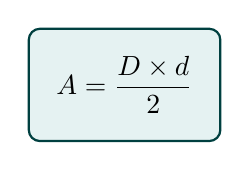
\begin{tikzpicture}
\node[rectangle, fill=teal!10, rounded corners, inner sep=10pt, draw=teal!50!black, thick] (box) {
$\displaystyle A = \frac{D \times d}{2}$
};
\end{tikzpicture}

\subsection*{Círculo}

\begin{center}
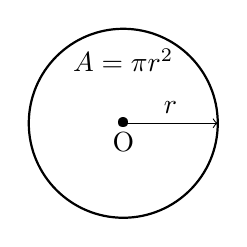
\begin{tikzpicture}[scale=0.8]
\draw[thick] (0,0) circle (1.5);
\draw[->] (0,0) -- (1.5,0) node[midway,above] {$r$};
\node at (0,0) {•};
\node at (0,0) [below] {O};
\node at (0,1) {$A = \pi r^2$};
\end{tikzpicture}
\end{center}

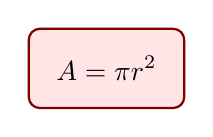
\begin{tikzpicture}
\node[rectangle, fill=red!10, rounded corners, inner sep=10pt, draw=red!50!black, thick] (box) {
$\displaystyle A = \pi r^2$
};
\end{tikzpicture}

\section*{Fórmulas para Polígonos Regulares}

\subsection*{Polígono Regular de $n$ lados}

\begin{center}
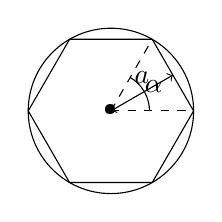
\begin{tikzpicture}[scale=0.7]
\draw (0:1.5) -- (60:1.5) -- (120:1.5) -- (180:1.5) -- (240:1.5) -- (300:1.5) -- cycle;
\draw[dashed] (0,0) -- (0:1.5);
\draw[dashed] (0,0) -- (60:1.5);
\draw (0:0.7) arc (0:60:0.7);
\node at (30:0.9) {$\alpha$};
\draw[<->] (0,0) -- (30:1.3) node[midway,above] {$a$};
\draw (0,0) circle (1.5);
\node at (0,0) {•};
\end{tikzpicture}
\end{center}

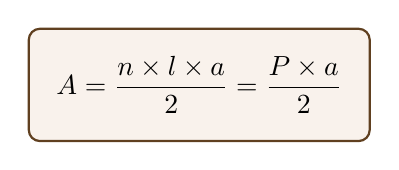
\begin{tikzpicture}
\node[rectangle, fill=brown!10, rounded corners, inner sep=10pt, draw=brown!50!black, thick] (box) {
$\displaystyle A = \frac{n \times l \times a}{2} = \frac{P \times a}{2}$
};
\end{tikzpicture}

\textbf{Onde:}
\begin{itemize}
\item $n$ = número de lados
\item $l$ = medida do lado
\item $a$ = apótema (distância do centro ao lado)
\item $P = n \times l$ = perímetro
\end{itemize}

\subsection*{Hexágono Regular}

\begin{center}
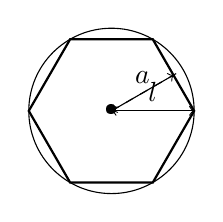
\begin{tikzpicture}[scale=0.7]
\draw[thick] (0:1.5) -- (60:1.5) -- (120:1.5) -- (180:1.5) -- (240:1.5) -- (300:1.5) -- cycle;
\draw[dashed] (0,0) -- (0:1.5);
\draw[dashed] (0,0) -- (30:1.5);
\draw[<->] (0,0) -- (0:1.5) node[midway,above] {$l$};
\draw[<->] (0,0) -- (30:1.3) node[midway,above] {$a$};
\draw (0,0) circle (1.5);
\node at (0,0) {•};
\end{tikzpicture}
\end{center}

\textbf{Fórmula especial:}
\[
A = \frac{3\sqrt{3} \times l^2}{2}
\]

\section*{Exercícios Básicos}

\begin{enumerate}[leftmargin=*]

\item Calcule a área das figuras:
\begin{enumerate}[label=\alph*)]
\item Quadrado com lado 5 cm
\item Retângulo com base 8 m e altura 3 m
\item Triângulo com base 10 cm e altura 4 cm
\end{enumerate}

\item Determine a área:
\begin{enumerate}[label=\alph*)]
\item Trapézio: $B = 12$ cm, $b = 8$ cm, $h = 5$ cm
\item Losango: $D = 16$ m, $d = 12$ m
\item Círculo: $r = 7$ cm ($\pi \approx 3,14$)
\end{enumerate}

\item Complete a tabela:

\begin{center}
\begin{tabular}{|c|c|c|c|}
\hline
\textbf{Figura} & \textbf{Dados} & \textbf{Fórmula} & \textbf{Área} \\
\hline
Quadrado & $l = 6$ m & $A = l^2$ & \\
\hline
Retângulo & $b = 15$ cm, $h = 4$ cm & $A = b \times h$ & \\
\hline
Triângulo & $b = 9$ m, $h = 6$ m & $A = \dfrac{b \times h}{2}$ & \\
\hline
Círculo & $r = 10$ cm & $A = \pi r^2$ & \\
\hline
\end{tabular}
\end{center}

\item Resolva os problemas:
\begin{enumerate}[label=\alph*)]
\item Um terreno quadrado tem 25 m de lado. Qual sua área?
\item Uma sala retangular mede 5 m por 4 m. Quantos m² de piso são necessários?
\item Um triângulo tem área 24 cm² e base 8 cm. Qual sua altura?
\end{enumerate}

\item Conversão de unidades:
\begin{enumerate}[label=\alph*)]
\item 2 m² = \underline{\hspace{1cm}} cm²
\item 5000 cm² = \underline{\hspace{1cm}} m²
\item 3 km² = \underline{\hspace{1cm}} m²
\end{enumerate}

\section*{Exercícios Intermediários}

\begin{enumerate}[leftmargin=*, start=6]

\item Calcule a área das figuras compostas:

\begin{center}
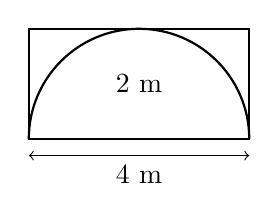
\begin{tikzpicture}[scale=0.7]
% Retângulo com semicírculo
\draw[thick] (0,0) rectangle (4,2);
\draw[thick] (4,0) arc (0:180:2);
\node at (2,1) {2 m};
\draw[<->] (0,-0.3) -- (4,-0.3) node[midway,below] {4 m};
\end{tikzpicture}
\end{center}

\begin{enumerate}[label=\alph*)]
\item Calcule a área total
\item Se o semicírculo fosse removido, qual seria a área restante?
\end{enumerate}

\item Triângulo com lados 5 cm, 6 cm e 7 cm:
\begin{enumerate}[label=\alph*)]
\item Calcule o semiperímetro
\item Use a fórmula de Herão para calcular a área
\end{enumerate}

\item Hexágono regular:
\begin{enumerate}[label=\alph*)]
\item Lado = 4 cm, calcule a área usando $A = \dfrac{3\sqrt{3} \times l^2}{2}$
\item Calcule o apótema (use $a = \dfrac{l\sqrt{3}}{2}$)
\item Verifique usando $A = \dfrac{P \times a}{2}$
\end{enumerate}

\item Comparação de áreas:
\begin{enumerate}[label=\alph*)]
\item Quadrado de lado 6 cm vs círculo de raio 3 cm
\item Triângulo de base 10 cm e altura 8 cm vs retângulo 5 cm × 8 cm
\end{enumerate}

\item Problemas contextualizados:
\begin{enumerate}[label=\alph*)]
\item Um tapete circular tem raio 1,5 m. Qual sua área?
\item Um terreno triangular tem base 30 m e altura 20 m. Qual seu valor se o m² custa R\$ 200?
\item Quantos ladrilhos quadrados de 20 cm de lado são necessários para cobrir uma sala de 4 m × 3 m?
\end{enumerate}

\end{enumerate}

\section*{Exercícios Avançados}

\begin{enumerate}[leftmargin=*, start=11]

\item Demonstre as fórmulas:
\begin{enumerate}[label=\alph*)]
\item Demonstre que $A = \dfrac{b \times h}{2}$ para triângulos
\item Mostre que $A = \dfrac{D \times d}{2}$ para losangos
\item Prove que $A = \pi r^2$ para círculos
\end{enumerate}

\item Relação entre áreas:
\begin{enumerate}[label=\alph*)]
\item Mostre que a área de um paralelogramo é o dobro da área de um triângulo com mesma base e altura
\item Prove que a área de um quadrado é metade da área do quadrado de sua diagonal
\end{enumerate}

\item Polígono regular inscrito:
\begin{enumerate}[label=\alph*)]
\item Para um polígono regular de $n$ lados inscrito em círculo de raio $R$, mostre que:
  \[
  A = \frac{nR^2 \sin\left(\frac{360^\circ}{n}\right)}{2}
  \]
\item Calcule para $n=4$ (quadrado) e $n=6$ (hexágono)
\end{enumerate}

\item Área por coordenadas:
\begin{enumerate}[label=\alph*)]
\item Dados vértices $(x_1,y_1), (x_2,y_2), (x_3,y_3)$ de um triângulo, mostre que:
  \[
  A = \frac{1}{2}|x_1(y_2-y_3) + x_2(y_3-y_1) + x_3(y_1-y_2)|
  \]
\item Calcule a área do triângulo com vértices (0,0), (4,0), (0,3)
\end{enumerate}

\item Máximos e mínimos:
\begin{enumerate}[label=\alph*)]
\item De todos os retângulos com perímetro 20 cm, qual tem maior área?
\item De todos os triângulos com base 10 cm e perímetro 24 cm, qual tem maior área?
\end{enumerate}

\item Áreas semelhantes:
\begin{enumerate}[label=\alph*)]
\item Se dois polígonos são semelhantes com razão $k$, qual a razão entre suas áreas?
\item Um triângulo tem área 12 cm². Qual a área de um triângulo semelhante com lados 50\% maiores?
\end{enumerate}

\item Problema histórico:
\begin{enumerate}[label=\alph*)]
\item Como Arquimedes aproximou a área do círculo?
\item Explique o método da exaustão
\end{enumerate}

\item Integral e área:
\begin{enumerate}[label=\alph*)]
\item Mostre que a área sob a curva $y = x$ de 0 a 1 é 0,5
\item Relacione com a área do triângulo
\end{enumerate}

\item Área de setor circular:

\begin{center}
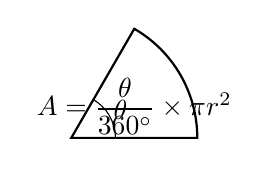
\begin{tikzpicture}[scale=0.8]
\draw[thick] (0,0) -- (2,0) arc (0:60:2) -- cycle;
\draw (0:0.7) arc (0:60:0.7);
\node at (30:0.9) {$\theta$};
\node at (1,0.5) {$A = \dfrac{\theta}{360^\circ} \times \pi r^2$};
\end{tikzpicture}
\end{center}

\begin{enumerate}[label=\alph*)]
\item Deduza a fórmula
\item Calcule a área de um setor de 90° em círculo de raio 4 cm
\end{enumerate}

\item Desafio final:
\begin{enumerate}[label=\alph*)]
\item Um quadrado e um círculo têm mesma área. Qual a razão entre seus perímetros?
\item Encontre todas as figuras com mesma área e perímetro
\end{enumerate}

\end{enumerate}

\section*{Resumo das Fórmulas}

\subsection*{Figuras Básicas:}
\begin{itemize}
\item Quadrado: $A = l^2$
\item Retângulo: $A = b \times h$
\item Triângulo: $A = \dfrac{b \times h}{2}$
\item Paralelogramo: $A = b \times h$
\item Trapézio: $A = \dfrac{(B+b) \times h}{2}$
\item Losango: $A = \dfrac{D \times d}{2}$
\item Círculo: $A = \pi r^2$
\end{itemize}

\subsection*{Polígonos Regulares:}
\[
A = \frac{P \times a}{2} = \frac{n \times l \times a}{2}
\]

\subsection*{Triângulo (outras fórmulas):}
\begin{itemize}
\item Herão: $A = \sqrt{p(p-a)(p-b)(p-c)}$
\item Lados e ângulo: $A = \dfrac{ab\sin\theta}{2}$
\item Coordenadas: $A = \frac{1}{2}|x_1(y_2-y_3)+x_2(y_3-y_1)+x_3(y_1-y_2)|$
\end{itemize}

\section*{Dicas para Cálculo}

\begin{itemize}
\item \textbf{Desenhe a figura}: Ajuda na visualização
\item \textbf{Identifique medidas}: Base, altura, raio, etc.
\item \textbf{Use unidades consistentes}: Todas na mesma unidade
\item \textbf{Verifique fórmulas}: Certifique-se de usar a correta
\item \textbf{Faça estimativas}: Verifique se resultado é razoável
\item \textbf{Use $\pi$ adequadamente}: 3,14 para aproximações
\end{itemize}

\section*{Aplicações Práticas}

\begin{itemize}
\item \textbf{Construção civil}: Área de terrenos e cômodos
\item \textbf{Agricultura}: Área de plantio
\item \textbf{Design}: Superfície de objetos
\item \textbf{Esportes}: Dimensões de quadras e campos
\item \textbf{Arquitetura}: Projetos de espaços
\end{itemize}

\end{multicols}

\end{document}
